\documentclass{beamer}

\usepackage{xspace}

 \usepackage{calc}                                             %%
    \usepackage{multirow}                                         %%
    \usepackage{hhline}                                           %%
    \usepackage{ifthen}   
    
\newcounter{saveenumi}
\newcommand{\seti}{\setcounter{saveenumi}{\value{enumi}}}
\newcommand{\conti}{\setcounter{enumi}{\value{saveenumi}}}                                      

\setbeamertemplate{caption}[numbered]{}
    
\providecommand{\pr}[1]{\ensuremath{\Pr\left\{#1\right\}}}
\providecommand{\brak}[1]{\ensuremath{\left(#1\right)}}
\providecommand{\cbrak}[1]{\ensuremath{\left\{#1\right\}}}
\providecommand{\sbrak}[1]{\ensuremath{{}\left[#1\right]}}


% Theme choice:
\usetheme{CambridgeUS}

% Title page details: 
\title{ASSIGNMENT 9 : PAPOULLIS CHAPTER : 4 EXAMPLE - 4.9} 
\author{AI21BTECH11016}
\date{\today}
\logo{\large \LaTeX{}}


\begin{document}

% Title page frame
\begin{frame}
    \titlepage 
\end{frame}

% Remove logo from the next slides
\logo{}

% Outline frame
\begin{frame}{Outline}
    \tableofcontents
\end{frame}

% Outline frame
\section{Question}
\begin{frame}{Question}
\begin{block}{}
A fair coin is tossed twice, and let the random variable \textbf{x} represent the number of
heads. Find $F_X(x)$.
\end{block}
\end{frame}

\section{Solution}
\begin{frame}{Solution}
The possible outcomes for the given random variable are : \\
\centering
\textbf{X} = \cbrak{HH, HT, TH, TT}\\
\begin{block}{}
\centering
x$\brak{HH}$ = 2\\ 
x$\brak{HT}$ = 1\\
x$\brak{TH}$ = 1\\
x$\brak{TT}$ = 0
\end{block}
\end{frame}

\begin{frame}
For x $<$ 0 :
\begin{align}
\cbrak{X\leqx} & = \emptyset \\ \Rightarrow F_X(x) & = 0 
\end{align}
For 0 $\leq$ x $<$ 1 :
\begin{align}
\cbrak{X \leq x} & = \cbrak{TT} \\ \Rightarrow F_X(x)& = \pr{TT} = \pr{T} \pr{T} = \frac{1}{4}
\end{align}
For 1 $\leq$ x $<$ 2 :
\begin{align}
\cbrak{X \leq x} & = \cbrak{TT, HT, TH} \\ \Rightarrow F_X(x)& = \pr{TT} + \pr{HT} + \pr{TH} = \frac{3}{4}
\end{align}
\end{frame}

\begin{frame}
For x $\geq$ 2 :
\begin{align}
\cbrak{X \leq x} & = X \\ \Rightarrow F_X(x)& = 1
\end{align}

\end{frame}

\begin{frame}{Graph of $F_x(x)$}
        \centering
        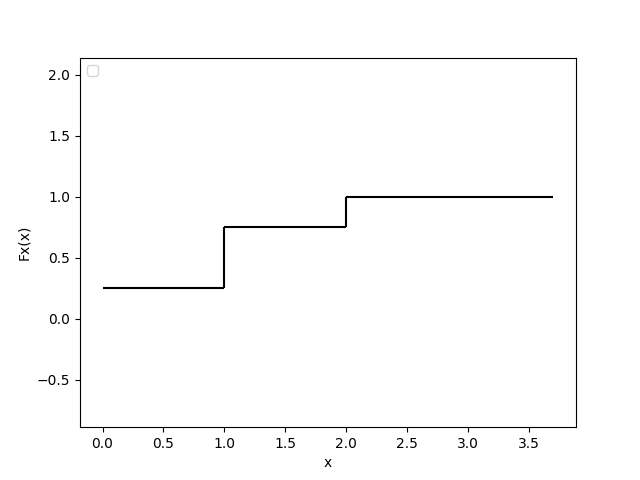
\includegraphics[height=0.8\paperheight]{images/image9.png}     
\end{frame}

\end{document}